In this chapter, we provide detailed information regarding the design of our modular framework, as well as its implementation.

\section{BlockLearning Framework's Design}\label{framework:design}

The modular framework, to which we called BlockLearning, is designed in such a way that modules can be added, as well as removed or changed, easily. In this framework, the devices, identified by the address of their account in the blockchain, can be classified into three categories: \textit{trainers}, \textit{aggregators} and \textit{scorers}. Additionally, the entity that deploys the contract and is responsible for starting and terminating the rounds is called \textit{model owner}.

A device, i.e., a client or a server, can be categorized as one or more categories. For example, BlockFlow's scoring algorithm is executed by the clients, which are then categorized as trainers and scorers, while the servers are categorized as aggregators. In contrast, Multi-KRUM is executed by the servers, which are then categorized as aggregators and scorers, while the clients are categorized as trainers. By allowing each device to play more than one role, the framework provides flexibility to support different architectures and algorithms.

\begin{figure}[!ht]
    \centering
    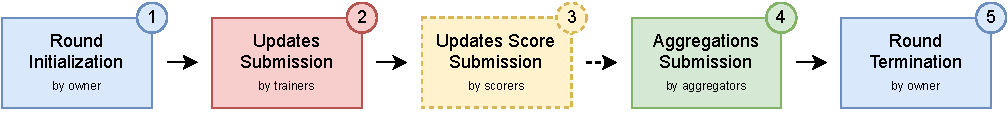
\includegraphics[width=1\textwidth]{graphics/sequence.pdf}
    \caption{BlockLearning's Execution Flow}
    \label{fig:blocklearning_steps}
\end{figure}

The framework supports a modular sequential flow represented in \autoref{fig:blocklearning_steps}. This flow is based on the current literature and the steps required to perform the Federated Learning process via the blockchain. The steps are explained below:

\begin{enumerate}
    \item The model owner initializes the round. During the round initialization, depending on the participant selection algorithm, the trainers that will participate may have been selected already, or not.
    
    \item The trainers retrieve the information such as the global weights from the last round and train the model using their local data. Then, the trainers submit their model updates.
    
    \item If a scoring algorithm is enabled, the scorers retrieve the updates and calculate the scores. Then, they submit their scores.
    
    \item The aggregators retrieve the model updates and execute the aggregation algorithm and submit the aggregation results to the blockchain.
    
    \item Finally, the model owner sends a transaction to the blockchain in order to terminate the round. At this point, the smart contract checks if the majority of the aggregators agreed on the aggregation. If so, the round is marked as terminated. Otherwise, the round fails, indicating that the aggregators did not reach an agreement, which may indicate that some of the aggregators are compromised.
\end{enumerate}

In the last step of the execution flow, the smart contract checks if the majority of the aggregators agree on the aggregation. The majority is defined by \textit{at least 50\%}. Therefore, the framework offers a 50\% threat model. However, the threat threshold can be changed, changing the threat model.

\subsection{Structure and Modules}\label{meth:struct_modules}

The framework is divided into three main software components: the smart contracts, the library, and the testbed. The structure of the framework, as well as its components and their corresponding modules, is depicted on \autoref{fig:blocklearning_modules}. Each of the components plays a different role in the overall system in order to support the logical flow shown in \autoref{fig:blocklearning_steps}. In the following subsections, each of the components will be explained in more detail.

\begin{figure}[!ht]
    \centering
    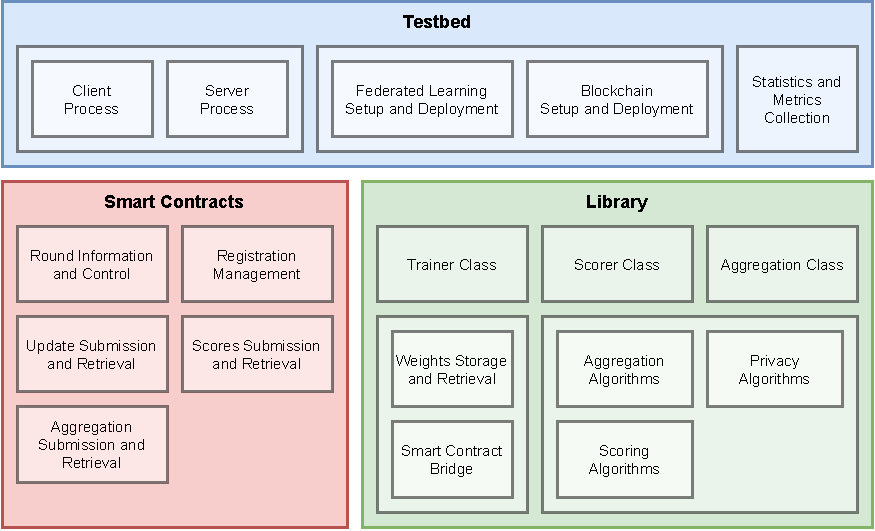
\includegraphics[width=1\textwidth]{graphics/modules.pdf}
    \caption{BlockLearning's  Structure and Modules}
    \label{fig:blocklearning_modules}
\end{figure}

\subsubsection{Smart Contracts}\label{meth:smart_contracts}

The first component of the framework is the smart contracts. The smart contracts live on the blockchain and are the main means of communication between FL clients and servers. In addition, the smart contracts hold information regarding the current status of the round, as well as the updates, scores, aggregations, among others. The smart contracts provide the following functionality:

\begin{itemize}
    \item \textit{Round Information and Control}: the smart contract must provide information on whether the round is ongoing and which phase, i.e., scoring, aggregation, or termination phase, it is in. It must allow for flexibility such that new phases can be added in the future, such as the backpropagation confirmation phase we need for our vertical model. In addition, it must allow for rounds to be started and marked as terminated. Round phase advancements are defined through pre-defined conditions that, once met, automatically move the round to the next phase. For example, after all updates are received, the smart contract should move to the next phase.
    
    \item \textit{Registration Management}: the smart contract must allow devices to register themselves as trainers, aggregators, or scorers in the system. Finally, the smart contract should provide information about which devices participate in each round.
    
    \item \textit{Update Submission and Retrieval}: the smart contract must allow trainers to submit their updates, which must include a pointer to the model weights and the amount of data points that were used to train the model. In addition, it can include the training accuracy and testing accuracy for each individual trainer. The submissions must be accessible.
    
    \item \textit{Scores Submission and Retrieval}: the smart contract must allow scorers to submit their scores. It must be possible to know which scorer scored which update and they must be accessible.
    
    \item \textit{Aggregation Submission and Retrieval}: the smart contract must allow aggregators to submit the aggregations, which contain a pointer to the weights. The aggregations must be accessible.
\end{itemize}

\subsubsection{Library}\label{meth:library}

The second component of the framework is the library. The library encodes the algorithms, utilities, and building blocks necessary to implement the scripts that run on the clients and the servers. It must include:

\begin{itemize}
    \item \textit{Aggregation, Scoring} and \textit{Privacy Algorithms}: implementation of the different algorithms. For each algorithm type, a common interface must be implemented, such that adding new algorithms is easy and simple and they are interchangeable.
    
    \item \textit{Weights Storage and Retrieval}: utilities to load and store weights on the decentralized storage provider. These must also provide an interface in order to make it easy to change the storage provider by providing a different implementation.
    
    \item \textit{Smart Contract Bridge}: a contract class that provides an interface to the smart contract that lives on the blockchain. With this class, it should be possible to call the smart contract functions as if they were local functions.
    
    \item \textit{Trainer, Scorer} and \textit{Aggregator Classes}: a class per each device category. This class must register the devices as their category upon initialization. It must also provide methods to execute the training, scoring and aggregation tasks, respectively.
\end{itemize}

\subsubsection{Testbed}\label{meth:testbed}

The third component of the framework is the testbed. The testbed provides the platform to conduct the experiments in a reproducible way, for instance by setting static seeds for randomness. The testbed must include:

\begin{itemize}
    \item \textit{Client, Server} and \textit{Owner Scripts}: scripts that will be run at the clients, the servers, and at the model owner, respectively. These scripts will use the library in order to perform the right tasks according to which algorithm is being used.
    
    \item \textit{Federated Learning Setup and Deployment}: scripts and tools to easily deploy the client and server machines in a test environment, such as containers.
    
    \item \textit{Blockchain Setup and Deployment}: scripts and tools to easily deploy the blockchain network in a test environment using the different consensus algorithms, and to deploy the contract to such network.
\end{itemize}

In addition, the testbed must also include tools to collect the required statistics and logs that can be later processed to retrieve the metrics necessary for the impact analysis.

\section{BlockLearning Framework's Implementation}

In this section, we go over the implementation details of the BlockLearning framework, following the guidelines defined in \Cref{framework:design}. The complete implementation is publicly available on GitHub\footnote{\url{https://github.com/hacdias/blocklearning}}.

\subsection{Smart Contracts}

As mentioned previously, we use the Ethereum \cite{wood2014ethereum} blockchain platform as it is the most popular and compatible with all the techniques we use for our experiments and comparison with the related work. Therefore, the smart contracts must be implemented in a programming language that supports Ethereum. We chose the Solidity \cite{solidity} programming language as it is the most well-known with the widest support.

Since our framework supports different algorithms, we need four different smart contracts. These smart contracts inherit most of their functionality from an abstract smart contract that provides the common data structures and functionality, named \texttt{Base}. Then, we implement the following classes, that derive from \texttt{Base}:

\begin{itemize}
    \item \texttt{RandomSelectionNoScoring}, which is used when we do not need a scoring algorithm. It only adds a new function to the \texttt{Base} class in order to allow the model owner to start a round with random participant selection.
    
    \item \texttt{RandomSelectionScoring}, which is used when we need a scoring algorithm. This smart contract implements the required methods to support the scoring phase, such as scoring submissions and the scoring round. In addition, it adds a function to allow the model owner to start a round with random participant selection.
    
    \item \texttt{FirstComeFirstServedNoScoring}, which is used with the first-come first-served participant selection algorithm with no scoring mechanism. It adds a function to allow the model owner to start a round with first-come first-served participant selection.
\end{itemize}

A class diagram with the public interfaces of the contracts, as well as the data types, is depicted in \autoref{fig:contracts-uml}. From the diagram, we can see that the smart contract provides round information and control, registration management, updates submission and retrieval, scores submission and retrieval, as well as aggregation submission and retrieval. One may note that the scores submission and retrieval are only implemented in \texttt{RandomSelectionScoring} as the remaining smart contracts are not used with scoring mechanisms.

\begin{figure}[!ht]
    \centering
    \centering
    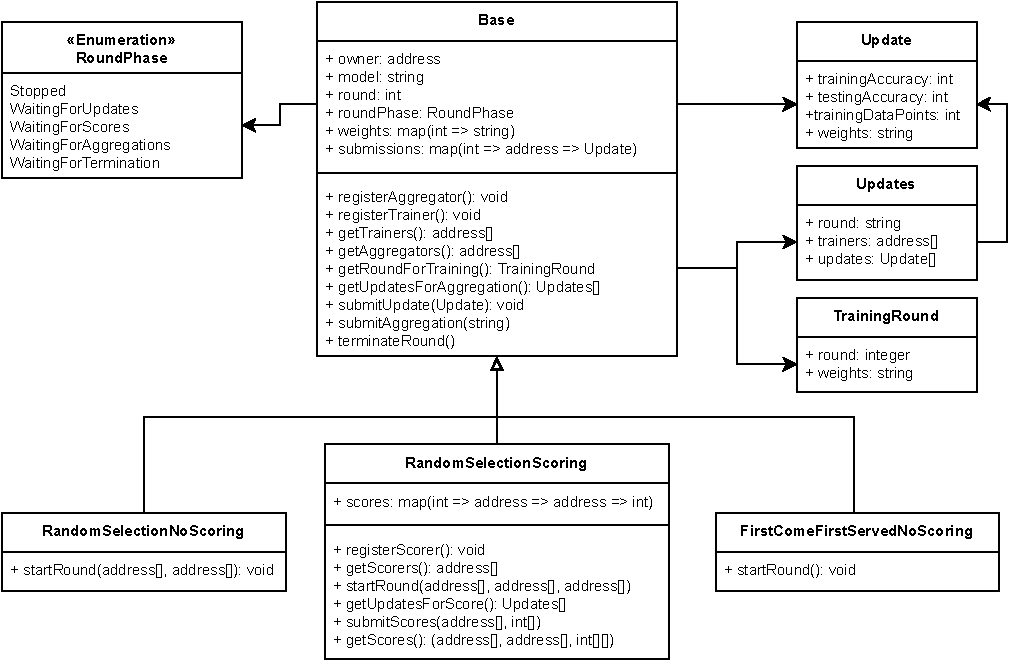
\includegraphics[width=1\textwidth]{graphics/smart-contract-uml.pdf}
    \caption{Smart Contracts Class Diagram}
    \label{fig:contracts-uml}
\end{figure}

An interesting implementation detail to note is that score and accuracy values are stored as integers. Currently, Solidity does not support floating point numbers. To preserve fidelity, the original values are multiplied by a large integer, $10^{18}$. Then, when the values are retrieved from the smart contract, they are divided by the same value in order to get the original value.

\subsection{Library}

The library is implemented in the Python \cite{10.5555/1593511} programming language. The main motivation for using Python is that many well-known Machine Learning libraries, such as TensorFlow \cite{tensorflow2015-whitepaper} and PyTorch \cite{NEURIPS2019_9015} are implemented in Python, as well as many data processing tools.

\subsubsection{Aggregation, Scoring and Privacy Algorithms}

The first component of the library is the aggregation, scoring and privacy algorithms. Each of these categories of algorithms has a specific interface to which each algorithm must conform to. By having a common interface, we can implement new algorithms, or change existing ones, easily. The interfaces are as follows:

\begin{itemize}
    \item \texttt{aggregate(trainers, updates, scorers, scores) $\rightarrow$ weights}\\
    The aggregators must provide a function \texttt{aggregate} that receives an array with the trainer addresses, an array with the updates sorted by the same order as the trainers, an array with the scorers and an array with the scores sorted by the same order as the scorers. It is important to note that the scorers and the scores are optional arguments since a scoring algorithm is not always required. The function returns an array with the aggregated weights. % BlockFlow, FedAvg, Multi-KRUM
    
    \item \texttt{score(round, trainers, updates) $\rightarrow$ trainers, scores}\\
    The scorers must provide a function \texttt{score} that receives an integer with the round number, an array with the trainer addresses, as well as an array of updates that are sorted by the same order as the trainer addresses. The function returns an array with the trainers and their submission scores. % Multi-KRUM, MarginalGain, Accuracy (BlockFlow)
    
    \item \texttt{privatize(x) $\rightarrow$ y}\\
    The privacy mechanisms must provide a function \texttt{score} that receives an array of the weights \texttt{x} and returns the privatized weights \texttt{y}. % Gaussian
\end{itemize}

Each of the aggregation and scoring algorithms is implemented based on the algorithms and details provided by the original authors. The local differential privacy is implemented using IBM's \texttt{diffprivlib} \cite{diffprivlib} library.

\subsubsection{Weights Storage and Retrieval}

The second component of the library is the utilities to store and retrieve the weights. The weights storage class also provides a common interface such that it is possible to change which storage provider we use. For our implementation, we use the InterPlanetary File System (IPFS) \cite{10.48550/arxiv.1407.3561} as our decentralized storage provider since it was used by many of the works reviewed in \Cref{chapter:related_work}.

IPFS is a distributed content addressed file system, which implies that, every file is addressed by its content. It works by attributing a hash, based on the file's content. Using this hash, also known as Content Identifier (CID), the file can be retrieved from the network and guaranteed to be immutable. Instead of storing the entire file in the blockchain, the CID can be stored. Pairing IPFS with the blockchain keeps the system decentralized and distributed, while offloading the storage to a different system.

\subsubsection{Smart Contract Bridge}\label{impl:bridge}

The third component is the smart contract bridge class. The smart contract bridge is implemented using the \texttt{Web3.py} \cite{web3py} library, which provides utilities to call the functions of the smart contracts. The contract bridge class provides 1:1 functions for each functions of the smart contract.

\subsubsection{Trainer, Scorer and Aggregator Classes}

The fourth and the final component of the library is the \texttt{Trainer}, \texttt{Scorer} and \texttt{Aggregator} classes. These classes implement the main flow of each of these procedures using the modules aforementioned described. For example, the trainer class is initialized with the contract bridge, the weights storage, the model, the data and an optional privacy mechanism. Then, it provides a method \texttt{train()} that executes the training procedure. Similarly, the scorer class provides \texttt{score()} and the aggregator class provides \texttt{aggregate()}.

\subsection{Testbed}

The testbed, that is, the platform to conduct the experiments. It was mostly implemented using the aforementioned library and Docker \cite{docker}. Docker is a platform that allows to easily deploy applications in an isolated setting through what is called a container, allowing us to simulate multiple devices in the same network. Each container runs an image, which is the name given to the piece of software than runs on the container.

In the testbed, we have two major components: the client, server and model owner scripts, the federated learning environment deployment and the blockchain deployment. These are discussed on the following subsections.

\subsubsection{Client, Server and Owner Scripts}

The client, server and model owner scripts are the processes that will run at the client, server and model owner, respectively. These are implemented using the BlockLearning library. In each of these scripts, we first load the required data, such as the data set in the clients, and initialize the required algorithms, namely the scoring, aggregation and privacy algorithms.

Then, depending on the scoring algorithm, we initialize the relevant classes at the correct machines. For example, for the BlockFlow scoring algorithm, the client initializes a \texttt{Trainer} and a \texttt{Scorer}, while the server initializes an \texttt{Aggregator}. In contrast, for Multi-KRUM, the client only initializes a \texttt{Trainer}, while the server initializes an \texttt{Aggregator} and a \texttt{Scorer}. On \autoref{alg:client_loop} you can visualize part of the main loop of the client script.

\begin{algorithm}
\caption{Client Script Main Loop}\label{alg:client_loop}
\begin{algorithmic}
\Require $s \in$ \{\O, BlockFlow, MarginalGain\}
\State $T \gets $ Initialize Trainer
\If{$s$ is not \O}
    \State $S \gets $ Initialize Scorer
\EndIf
\While{True}
    \State $P \gets$ Get Phase From Smart Contract
    \If{$P$ is Waiting For Updates}
        \State Execute Training Procedure $T.train()$
    \ElsIf{$P$ is Waiting For Scores}
        \State Execute Scoring Procedure $S.score()$
    \EndIf
\EndWhile
\end{algorithmic}
\end{algorithm}

\subsubsection{Blockchain Setup and Deployment}

The Blockchain setup and deployment is done using already existing tools and our library. As previously mentioned, we use Docker containers in order to run the experiments. Moreover, we use Docker Compose in order to deploy multiple containers at once and orchestrate the deployment process.

We use different Ethereum implementations, depending on the consensus algorithm since they are not all available within the sample implementation. Ethereum's main implementation, \texttt{go-ethereum} \cite{go-ethereum}, provides PoA and PoW. For QBFT, we use a fork called \texttt{quorum} \cite{quorum}, which is mostly identical to \texttt{go-ethereum} but supports QBFT.

Moreover, the Blockchain setup and deployment follows the following steps:

\begin{enumerate}
    \item \textit{Generate Accounts}. In first place, the Ethereum accounts for the clients and servers are generated using the provided \texttt{go-ethereum} toolkit. Each account is pre-loaded with $100$ ETH, the Ethereum currency, so that clients or servers will not run out of currency to submit their transactions.
    
    \item \textit{Build Images}. In second place, we build the Docker images that will be used to deploy the Blockchain network. This images are based on the images provided by each of the Ethereum's implementations that we use. In addition, they pre-load the account information, as well as some additional configuration to ensure that all nodes are connected when the network is bootstrapped.
    
    \item \textit{Deploy Network}. In third place, the network is deployed using Docker Compose and the configured amount of nodes.
    
    \item \textit{Deploy Contract}. Finally, the contract is deployed to the network using Truffle, which is a tool designed to help developers developing and deploying smart contracts.
\end{enumerate}

Finally, we would like to mention that originally we were planning on testing the PoS consensus algorithm. However, the only fork providing PoS support does not work in private network settings \cite{issuePos}. Therefore, it was not possible to run an experiment with PoS.

\subsubsection{Federated Learning Setup and Deployment}

Similarly to the Blockchain setup and deployment, we also use Docker Compose for the Federated Learning system. The process is identical as in the previous section, except that we only build the images and deploy the Federated Learning network.

\subsubsection{Statistics and Metrics Collection}

The different components of the library, such as the \texttt{Trainer}, \texttt{Scorer} and \texttt{Aggregator} classes, produce logs. These logs contain information related to timestamps and round number, and events that happen at certain points of the execution, such as: \textit{aggregation started}, \textit{aggregation ended}, \textit{scoring started}, \textit{scoring ended}, among others. These logs are retrieved from the containers using command-line tools implemented into a script called \texttt{toolkit.py}.

In addition, resource-related statistics, such as RAM usage, CPU usage, and network traffic, are collected directly from the Docker, through the \texttt{docker stats} command.
